%!TEX root = ../dissertation.tex
\chapter{Introduction}
\label{introduction}
Printed Electronics (PE) offers the flexibility to print electric components on diverse substrates, including not only traditional rigid materials like glass but also flexible materials like plastic foils~\cite{motivation1}. This adaptability makes PE particularly suitable for manufacturing a wide array of products, ranging from flexible keyboards and conformable antennas to interactive books, posters, and electronic skin patches.
Moreover, printed electronics (PE) introduces a paradigm shift in manufacturing of electronic devices, where the electronic components are fabricated by depositing functional materials on top of each other. The additive manufacturing processes used in PE results in lower fabrication costs, making it an intriguing prospect for applications where cost considerations outweigh the need for ultra-high device performance. The additive manufacturing methods are suitable to digitally fabricate microelectronic circuits. The development and commercialization of applications in printed electronics are of great interest on account of its continuously material improvement, waste reduction, and its promising ability to use a plethora of substrates, such as silicon, glass, textiles, and paper, amongst others.
Within the last decade, notable accomplishments in material optimization resulted in improved device characteristics, but additional research is imperative to enhance their electrical properties further. This includes elevating mobility and carrier densities to improve the properties of devices, such as transistors~\cite{motivation2}. However, it is important that transistor characteristics, such as the threshold voltages, are within a certain margin, so that the functionality of the circuits is satisfied. 
Optimizing the device characteristics will help to improve the yield of circuits. Thereby, curing conditions of the semiconducting indium oxide film is adjusted to improve the yield of logic gates, which is important for combinatorial and complex circuits. Based on NAND gates, adders, which are the main elements in arithmetic logic units, are attempted to be fabricated. This would allow for interesting novel applications where for instance sensor data could be directly evaluated next to the sensor, reducing noise which could pollute the sensor data.
Logic computing primarily emphasizes reasoning applications, such as central processing units and field-programmable gate arrays and there is an urgent demand for innovation in logic devices, characterized by decreased power consumption, and diversification of functional applications to sustain information processing capabilities. For that aim the state-of-the-art adder together with the half adder both are interesting to be fabricated to make the further complex computational sector such as Arithmetic Logic Unit (ALU) easier to be fabricated in the realm of printing electronics. 
This challenge can be mitigated before fabrication by better circuit designing for example using their NAND configuration which consume less transistors and through the fabrication by using optimised materials to ensure avoid any crossing and also systematically optimizing the unit device of the whole circuit to reach more total gain and determining the characteristics crucial in operation of a field-effect transistor to have a potentially promising EGFETs design.
Furthermore, logic gates were designed in Process Design Kit PDK in both their passive and active configurations to be fabricated. The advantage of using basic logic gates is to ensure the performance of the used materials and ensure the reliability of them.


In this chapter the author attempted to firstly introduce  printed electronics and then argued the substantial properties of $In_2O3$.
Furthermore, a quick review over the integrated circuits through the whole history of semiconductor in the satisfying well known moor’s law has been delivered.

\section{ Drop-on-Demand Inkjet Printed Electronics}
While the Si industry strives to miniaturize devices for improved performance, PE emphasis not on shrinking feature sizes but on the scalability of large-area applications. The concept of PE revolves around the on-demand and low-cost fabrication of electric circuits directly onto various substrates, such as glass or plastic foils. This approach stands in contrast to the intricate and precise manufacturing processes required in traditional Si technology.

The synergy between Si-based devices and printed electronics lies in their complementary rather than competition. Si-based field-effect transistors (FETs) excel in high-performance scenarios, with their superior field-effect mobility and well-established manufacturing processes. On the other hand, PE emerges as an attractive alternative in situations where manufacturing costs take precedence over individual device performance. The cost-effectiveness of PE stems from an additive fabrication process, in contrast to the subtractive processes common in Si technology , allowing the deposition of functional materials using affordable printing methods without the need for expensive masks.

From its beginning, printed electronics have employed various printing methods for the production of both active and passive components in electronic devices. Among various printing technologies, the inkjet printing method has been a main interest to industry because it can easily be scaled up for mass production.


In this method, referred to as inkjet printing, potential energy is utilized to propel ink, converting it into mechanical energy. This technique follows a 'drop on demand' approach, allowing precise dispensing of ink when necessary, without direct substrate contact. As depicted in the illustration \ref{fig9} and\ref{fig11}, a piezoelectric sheet linked to the nozzles is activated by an adaptable sinusoidal potential. The nozzle can be moved longitudinally to the substrate at a user-defined height. The sinusoidal potential influences the size and volume of the resulting droplet, facilitating controlled deposition of printed patterns. The droplet's configuration is also impacted by the nozzle diameter, typically around 20 μm, and the resulting drop volume is 10 pL, achieving printed resolutions as fine as 20 μm ~\cite{ref16}. The formation of droplets is pivotal since, in inkjet printing, individual drops collaboratively shape the desired pattern or configuration after deposition. The separation or coalescence of drops, known as drop spacing, between the centres of two printed drops is a critical factor. Hence, the drop diameter must conform to the acceptable range of drop spacing in the inkjet printer, ensuring consistent film formation during the drying process. Due to the fixed nozzle diameter, the drop size is generally controlled by the fluid properties of the ink.
\begin{figure}[h!]
\centering
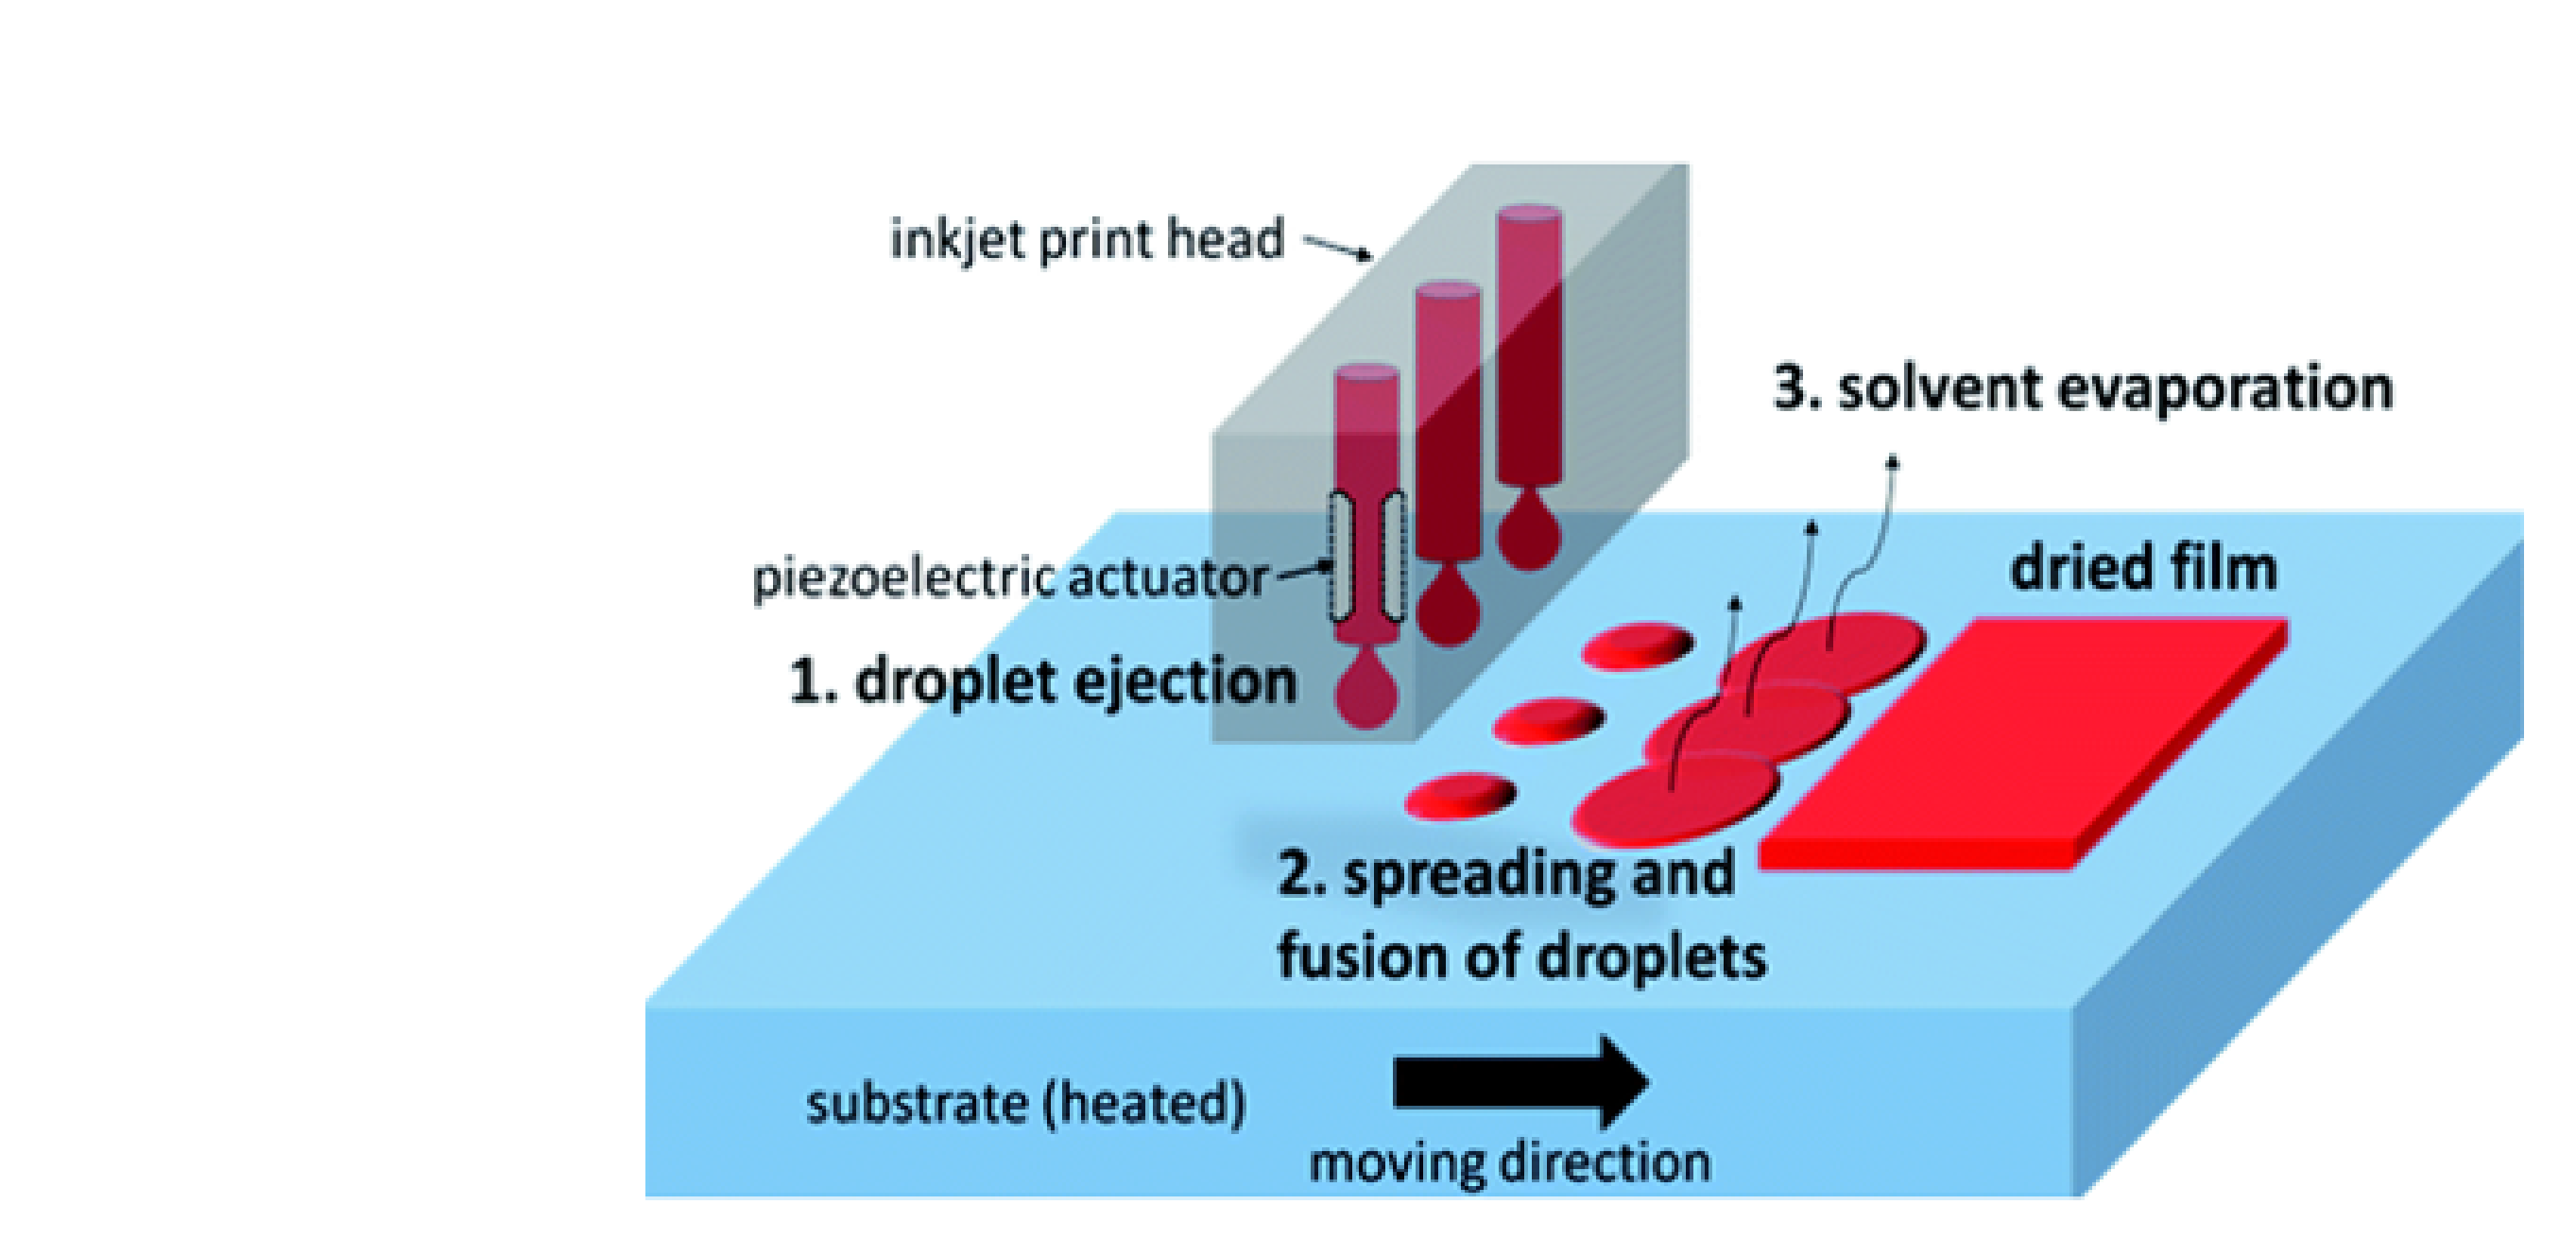
\includegraphics[width=1\textwidth]{figures/fig9.png}
\caption[Example of caption.]{The piezoelectric component linked to the nozzles may undergo mechanical strain upon the application of electrical potential for liquid ejection. The inkjet nozzle demonstrates movement in three dimensions concerning the substrate, and the precision of drop spacing influences the effective formation of the output. ~\cite{ref16}\label{fig9}}
\end{figure}

\begin{figure}[h!]
\centering
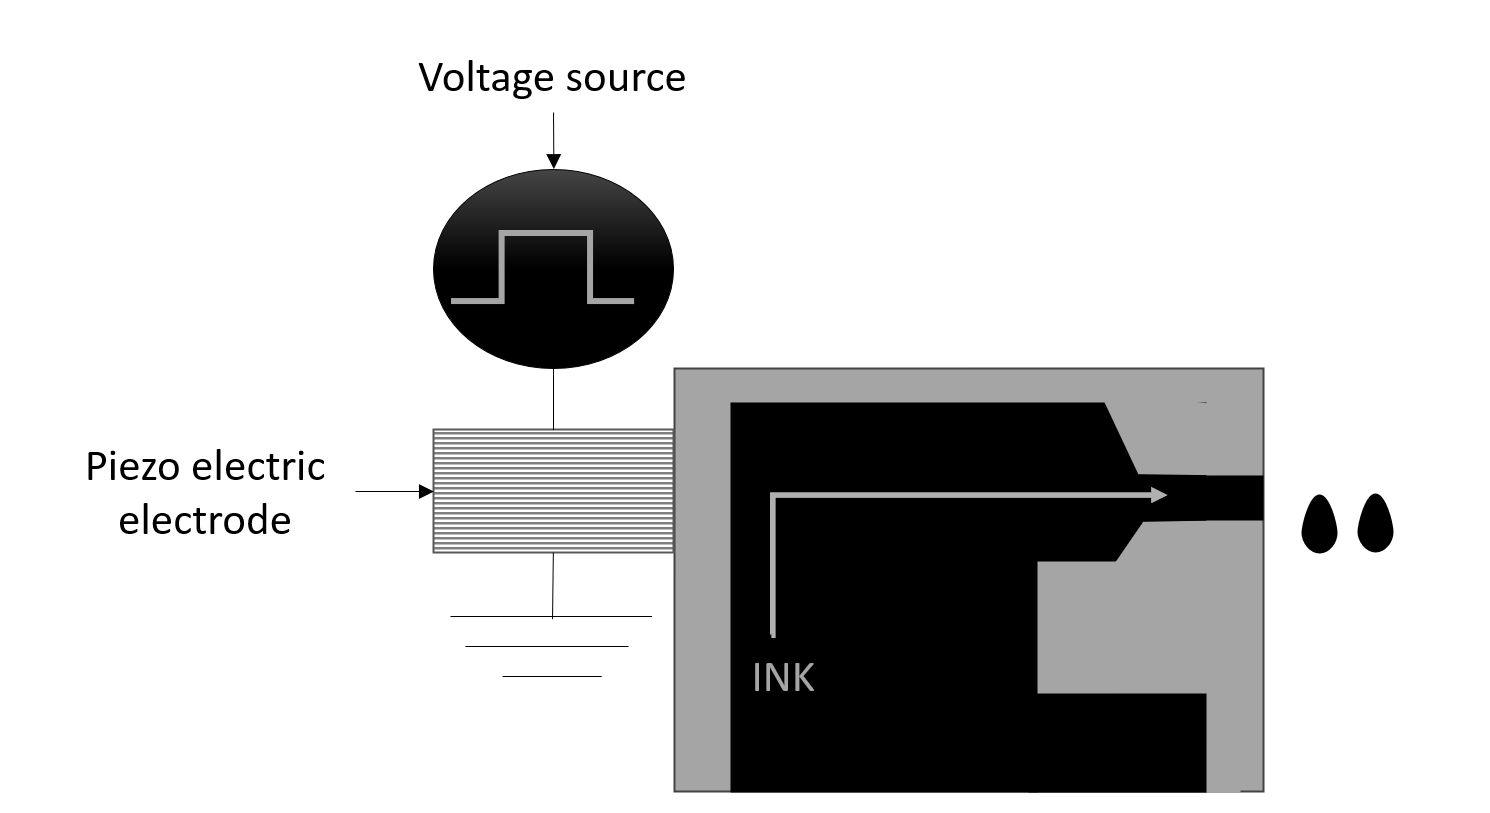
\includegraphics[width=1\textwidth]{figures/fig11.png}
\caption[Example of caption.]{ The schematic of a nozzle in inkjet printer \label{fig11}}
\end{figure}




In contemporary methods for depositing thin films, there is notable interest in non-contact approaches, particularly printing.
Various printing techniques can be broadly divided into two main categories: jetting and replication types. here some important properties of these methods have been mentioned ~\ref{tab:1}. Jetting-based technologies, such as inkjet printing, utilize a unique mechanism where ink is forced through a specialized nozzle. What sets this method apart is its digital and non-contact characteristics. The digital nature allows for meticulous control over printing patterns, providing high flexibility for diverse applications within the realm of PE. Additionally, the non-contact aspect of the inkjet printing process reduces the risk of contamination, enhancing the overall reliability and efficiency of printed electronic devices.

The printer head is a key element in this process. It  comprises of micrometer-scale nozzles for dispensing droplets. The mechanisms for ejecting ink fall into two categories: thermal inkjet involves heating and evaporating the ink solvent, while piezoelectric inkjet alters the nozzle shape through applied voltage ~\ref{fig11}. Various parameters such as diameter, temperature, and nozzle types play a direct role in shaping the morphology of the printed patterns.


The procedure involves the precise dispensing of small ink droplets onto the substrate . This droplets will flight and finally locate on the specific location on the  substrate. During this process, droplet's path can change by many parameters such as other drops, surface tension and last but not least based on the viscosity of the ink. ~\cite{ref27}

Also, surface properties such as the surface's energy, hydrophobicity or hydrifilicity effectively changed the printing shape.In the figure ~\ref{fig12} bellow there are different shaping of a printed line with same ink (same viscosity) and same (substrate) can be observed.

This can be roughly controlled by controlling the activation of a piezoelectric actuator, generating a pressure wave that propels the ink. 

One of the important challenges during printing is solidification of the ink according to the phase change of the material and makes both the speed of the printing and temperature applied to the nozzle important parameters. mechanism such as polymerization and evaporation occur due to these parameters and it highly is dependent on used ink. The setting for each material will be shown  later in  chapter ?  through the cartridge setting.
From the figure ~\ref{fig12} ~\cite{ref27}, different morphology of a printed line can be understand. All these types of morphologies also will be seen in the entire of this course due to the different condition in the printing days.
\begin{figure}[h!]
\centering
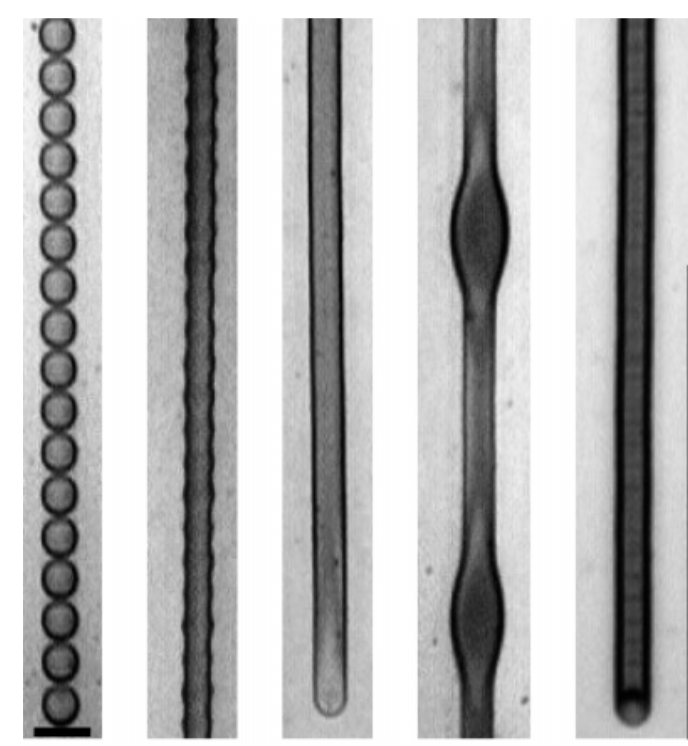
\includegraphics[width=0.5\textwidth]{figures/fig12.png}
\caption[Example of caption.]{Instances of fundamental behaviors exhibited by printed lines.\label{fig12}}
\end{figure}

~\cite{ref27} 





\begin{table}[h]
\centering
\caption{literature review of printing techniques }
\begin{tabular}{|c|c|c|c|c|}
\hline
& Inkjet & Arosel & Gravure & Screen \\
\hline
Printing  & Piezo & Engraved  & direct
writing using & Stencil  \\

form&controlled&cylinders& using&or\\

&& or rollers&  an aerosol spray &  screen mesh\\
\hline


Resolution &$ 2-50  \mu$ m & down to $10  \mu m $ & $2 \mu m$  & $100-300$  \\ 
&&&& dots  \\ 
&&&&per inch(dpi)   \\ 
\hline
Thickness & $100-500$ & $30-150$ & $10-400$ &$ 14000-25000$  \\
of film [nm] &&&&\\

\hline
\end{tabular}
\label{tab:1}
\end{table}


\section{Background and Related Works}
\label{Background and Related Works} 
\subsection{Metal-Oxide Semiconductors}
A bit of a history over a semiconductor prevails that it is actually fills the gap between physics and doing something which in practice is employed for the simplicity in our daily life and those applications can be summarized in three main groups as following: 1. Microelectronics devices 2. Optoelectronic devices and 3. Sensors. In the table presented below, significant milestones in the semiconductor's historical timeline are outlined.
\begin{table}[h]
\centering
\caption{literature review of semiconductor devices }
\begin{tabular}{|c|c|}
\hline
1874 & Braun discovers asymmetric\\ &conduction in semiconductor metal contacts\\
\hline
1906  & Pickard, point contact detector patent\\ 
\hline
1947  & Shockley Bardeen Brattain (Bell Labs) patent the first transistor in Ge\\ & (Nobel 1956)\\ 
\hline
1957  & Basov theorizes the semiconductor laser (Nobel 1964), it will be made by Hall in 1962.\\ & (It only worked at liquid nitrogen T)\\ 
\hline
1957  & Esaki: tunneling in semiconductors, tunneling diode (Nobel in 1973) \\ 
\hline
1958  &Kilby, first integrated circuits (IC),Texas instrument. (Nobel in 2000) \\ 
\hline
1965  & MOS transistor and CMOS IC (F. Faggin) Microelectronic borns \\ 
\hline
1968  &Alferov, Double eterostructure Laser (Nobel in 2000)…..Optoelectronics born.\\ & (It works at room T)\\ 
\hline
1969  & Boyle, Smith CCD invention (Nobel 2009)\\ 
\hline
1980  & Klaus von Klitzing , Quantum Hall effect (Nobel 1985)\\ 
\hline
1981  & Laughlin, Stomer, Tsue, Fractionary quantum Hall effect (Nobel 1998)\\ 
\hline
1989  & Blue light emitting diodes, Akasaki, Amano and Nakamura (Nobel 2014))\\ 
\hline
2004 & Geim, Novoselov : Graphene (Nobel 2010)\\ 
\hline
\end{tabular}
\label{tab:1}
\end{table}

One of the main classifications of semiconductors is based on their group numbers in the elemental periodic table. Some of these classifications are grouped as :
\begin{enumerate}
    \item Elemental semiconductors: Si, Ge in which all sites are occupied by same atom.
    \item Compound semiconductors (1:1 stoichimetry):
    \begin{itemize}
    \item III-V: Antimonides : AlSb, GaSb, InSb
    \item Aresides: AlAs, GaAs, InAs
    \item Phoshides: AlP, GaP, InP
    \item Nitrides: AlN, GaN, InN
    \item IV-IV: SiC
    \item II-VI: CdS, ZnS,ZnSe,ZnTe,MgS…
    \item II-VI CdSe,CdTe
    \item IV-VI PbSe, PbS,PbTe…
    \item Alloys
    \item Some Metal Oxydes TiO2, ZnO, CuO,InO….
\end{itemize}
\end{enumerate}
Circuits based on oxide semiconductors(Last Group) have shown promising results, demonstrating high stability under ambient conditions, lifetimes extending over several months, and overall high performance.
Common defects, like oxygen vacancies, formed during crystal growth or due to impurities, cause oxides to exhibit characteristics of either a p-type or n-type semiconductor due to the presence of defect states.
$In_2O_3$ is composed by metallic cations and oxide anions with ns° and $2s^2 2p^6$ valence electron configurations, respectively, and n = 5. 
In body-centred cubic bixbyite structure of $In_2O_3$  ~\cite{ref11}, the empty metallic s-orbitals,  constitute the conduction band minimum (CBM), while the valence band maximum (VBM) is composed by the filled oxygen $2$p-orbitals. If these materials were stoichiometric, $E_F$ would be in the middle of $E_g$, but the intrinsic and/or extrinsic defects take $E_F$ near or within the conduction band.
In the case of materials like$ In_2O_3$,  These vacancies act as charge carriers, contributing to the intrinsic n-type conductivity of the semiconductor.
\begin{figure}
    \centering
    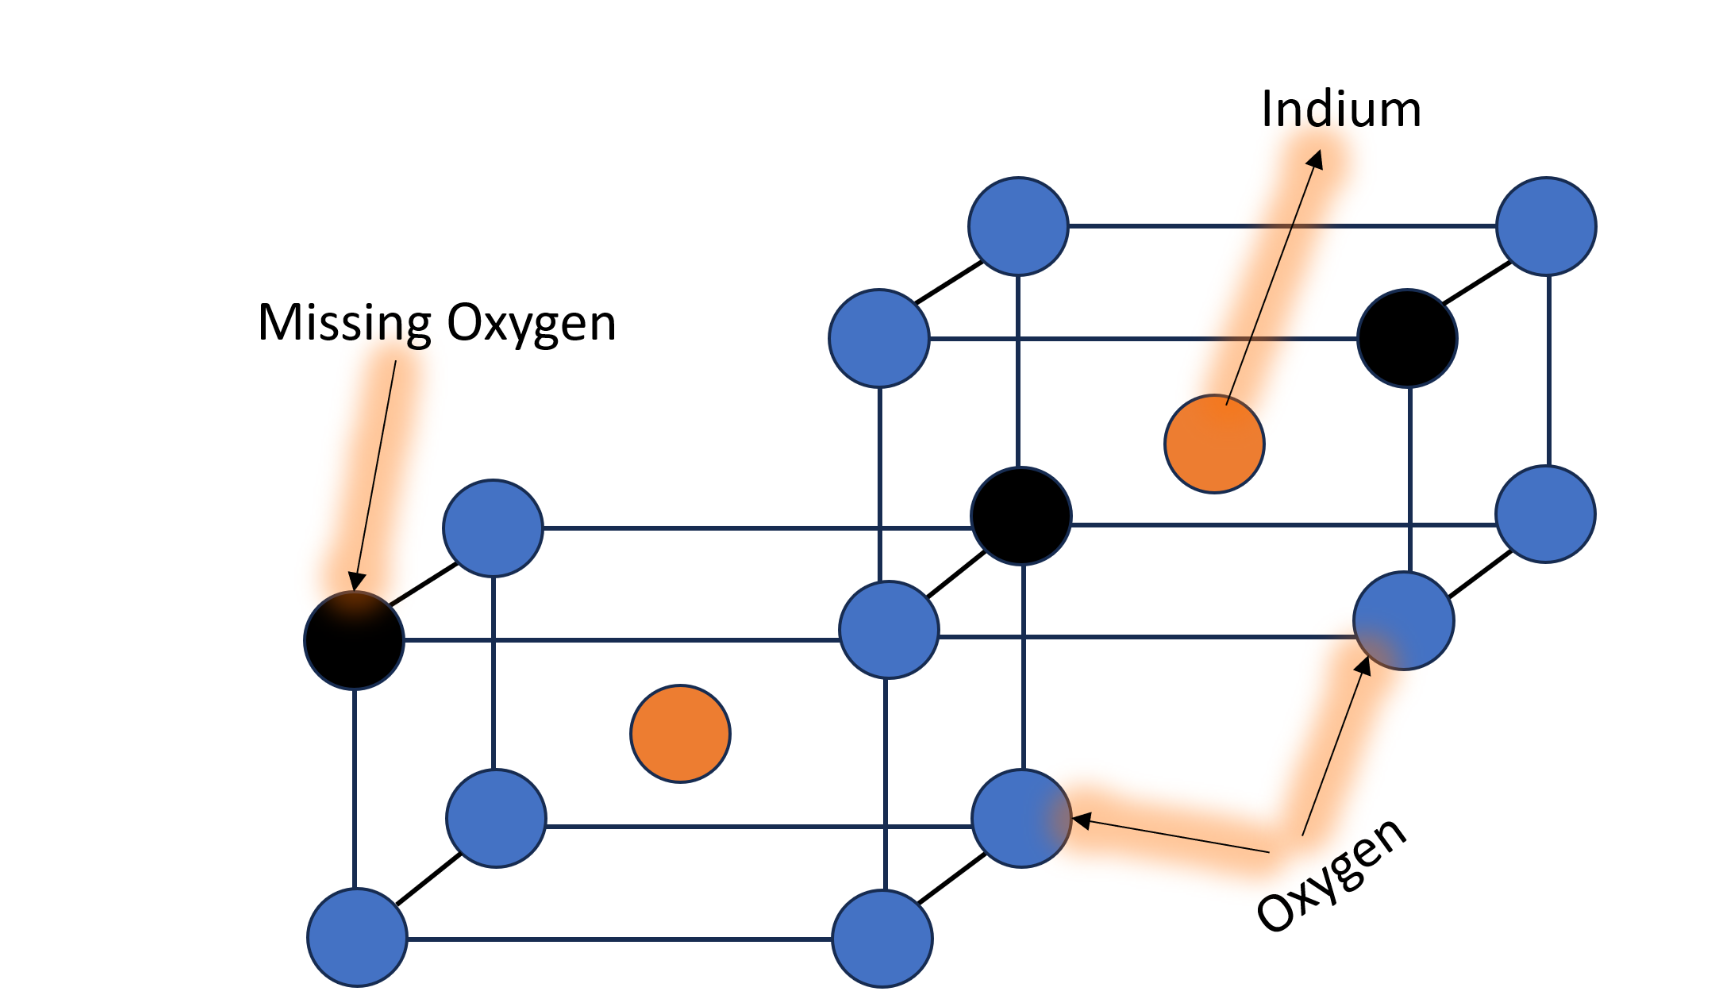
\includegraphics[width=0.7\textwidth]{figures/fig16.png}
    \caption{$In_2O_3$ structure with missing electrons providing free electrons leads to delocalized electrons inside crystal}
    \label{fig16}
\end{figure}

Recently, solution-processed oxide semiconductors such as indium oxide, indium gallium zinc oxide, and zinc oxide have gained popularity as channel materials in printed FET technology. 
Among these materials, Organic semiconductors, valued for their flexibility, are pivotal in printed electronics, but their carrier mobility must improve~\cite{ref27}. While high mobility in organics is often achieved with p-type materials, both n-type and p-type semiconductors are essential for CMOS-like logic circuits.  Inorganic semiconductors offer a broader selection of both p-type and n-type materials, enhancing versatility across electronic applications.

Compared to single crystal oxide semiconductors, which typically exhibit the highest carrier mobility values, indium oxide, demonstrates values in the range of several hundred $cm^2 V^{-1} s^{-1}$. This wide bandgap oxide semiconductors also possess advantageous properties such as stability in air across a broad temperature range, optical transparency, mechanical flexibility, ease of processability in printing techniques and non-toxic nature.

Furthermore, the array of electrodes available, indium tin oxide (ITO) stands out as the most widely utilized transparent electrode due to its exceptional qualities, combining high transmittance with low resistivity ($6.68\times 10^{–4} Ω cm$)~\cite{ref7}. ITO finds extensive application as an anode in various organic electronics, including organic light-emitting diodes and polymer solar cells, owing to its elevated work function characteristics. In this work for all the electrodes ITO has been used. ~\cite{ref8}

Indium oxide ($In_2o_3$), in particular, has garnered considerable interest as a semiconductor with a carrier concentration exceeding $10^{18} cm{⁻³}$ (depending on doping and preparation conditions), and an intrinsic mobility of 160 $cm{²} V{⁻¹} s{⁻¹}$ and a substantial band gap of (3.7 eV). ~\cite{ref1},  ~\cite{ref2}, ~\cite{ref3}.







\begin{table}[h]
\centering
\caption{Solution based inkjet printed n-type metal oxide TFTs: the channel material and electrical properties}
\begin{tabular}{|c|c|c|c|c|c|}
\hline 
\label{tab:3}
Channel 
&
Deposition 
&
 $ T_{max} $
&

{$\left[V dac^{-1}\right]$}
&
$I_{On}/I_{off} $
 & 
 Ref. 
 \\
material&method &°C&SS&ratio &\\
 \hline   IZO & Inkjet printing & 400  & - &-&~\cite{ref21} \\
 
\hline   IGZO & Inkjet printing & 350  & - &$10^7$&~\cite{ref20}  \\


\hline  $In_2O_3$ & Inkjet printing & 250 & 0.15 &$10^7$ & ~\cite{ref18} \\

\hline  $ZnO$ & Inkjet printing & 300  &0.75& $10^6$ & ~\cite{ref19}  \\

\hline  $ZIO$ & Thermal Inkjet  & 600  &-& $10^4$ &~\cite{ref22}  \\

\hline  $In_2O_3$ &  Piezoelectric   & 350  &-& $10^6$ & ~\cite{ref23}  \\

\hline
$In_2O_3$ &  Piezoelectric   & 150  &-& $10^6$ &~\cite{ref24}  \\

\hline
$In_2O_3$ &  Piezoelectric   & 225  &-& $10^6$ &~\cite{ref25}  \\

\hline
$In_2O_3$ &  inkjet printing& 300  &-& $1.122 * 10^6$ & This work \\

\hline
\label{tab:3}
\end{tabular}
\end{table}



\subsection {Low-Temperature Metal-Oxide Thin Film Transistors}  
TFTs, or three-terminal field-effect devices, operate similarly to traditional MOSFETs used in Silicon electronics. While in MOSFET technology, the substrate is a single crystal silicon wafer, which also serves as the active layerand needs high temperatures exceeding $1000$ degrees Celsius, TFTs are distinct as they are manufactured on insulating substrates like glass or plastic, using vacuum- or solution-processing ref deposition techniques  at lower temperatures$ <650^  { \circ} C$) .  
transistor typically having three terminals (with an additional fourth terminal in MOSFETs connected to the substrate), regulates channel resistance between two contacts. The channel's conductivity is controlled by the gate terminal, which creates an electric field, hence the term "field-effect." Carriers (electrons or holes) originate from the source terminal, serving as the entry point into the channel, and exit through the drain terminal. The voltage between the source and drain terminals determines the current flow through the channel. 
The key constituents of TFTs include IGFET, JFET, and MESFET, differentiated by their gate capacitor formation. IGFET employs an insulator, JFET and MESFET use the depletion layer of a p-n junction or a Schottky barrier, respectively. Further IGFET classifications include MOSFET/MISFET and HFET, with distinctions in insulator types. Despite MOSFETs being produced with various semiconductors and insulators, TFTs are notable for their manufacturing on insulating substrates, allowing for diverse applications in flexible and low-temperature electronics.

    \begin{figure}[h!]
\centering
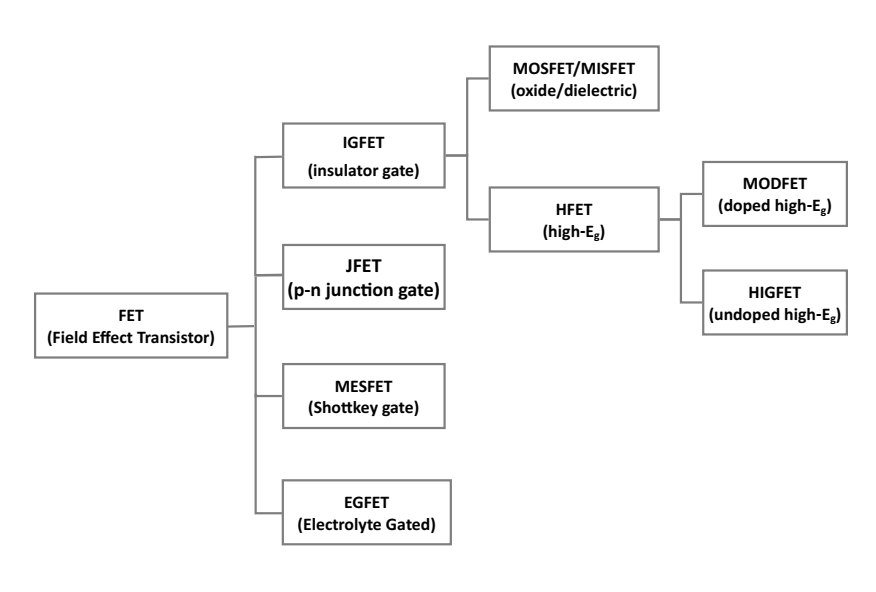
\includegraphics[width=1\textwidth]{figures/fig10.png}
\caption[Example of caption.]{Family tree of field-effect transistors (FETs) \label{fig14}}
\end{figure}
    

   \textit{MOSFET, JEFET and MESFET:}
   
The concept of the metal-oxide-semiconductor field-effect transistor (MOSFET) was initially introduced by Lilienfeld in the early 1930s and further explored by Shockley and Pearson in the late$ 1940$s. In$ 1960$, Ligenza and Spitzer achieved the first high-quality Si-SiO₂ MOS system through thermal oxidation. Atalla later proposed the fundamental MOSFET structure using this Si-SiO₂ system, with Kahng and Atalla reporting the first MOSFET in $1960$. 
The Junction Field-Effect Transistor (JFET), initially conceptualized and examined by Shockley in $1952$, primarily functions as a voltage-controlled resistor. Following Shockley's theoretical framework, the inaugural operational JFET was documented by Dacey and Ross. They subsequently explored the impact of field-dependent mobility on its functionality. In 1966, Mead introduced and showcased the Metal-Semiconductor Field-Effect Transistor (MESFET). Shortly thereafter, Hooper and Lehrer reported microwave performance in $1967$, utilizing a GaAs epitaxial layer on a semi-insulating GaAs substrate.
~\cite{ref14}

  \textit{EGFET}:
 
Garlapati et al. demonstrated the foundational principles for the construction of inkjet-printed electrolyte-gated transistors, also referred to as electrolyte-gated field-effect transistors (EGFETs), utilizing in-plane device structures ~\cite{ref73}. Subsequently, Marques et al. introduced classical top-gate bottom-contact stack Thin-Film Transistor (TFT) architecture for EGFETs as shown in Fig ~\ref{fig13}.
  \begin{figure}[h!]
\centering
\includegraphics[width=1\textwidth]{figures/fig13.png}
\caption[Example of caption.]{Side view of Electrolyte Gated Field Effect transistor's stacks  \label{fig13}}
\end{figure}
    

TFTs exhibit various device configurations, often featuring in-plane structures like coplanar architectures where the gate electrode, semiconductor layer, and source/drain electrodes are on the same surface. Coplanar TFTs commonly employ bottom-gate (BG) or top-gate (TG) architectures, depending on the sequence of gate electrode deposition relative to the active layer. 
\subsection {Electrolyte-gating }
\label{Electrolyte-gating}
Throughout the gate voltage application process, the transistor undergoes different stages such as accumulation and inversion within the transistor's operation such as enhancement or depletion mode.
Also, there are different regions where the transistor operates in, such as cut off, linear, or saturation regions that are existed based on the relationship between $V_{gs}$ and the threshold voltage $(V_{th})$.
If $V_{ds} ≤ V_{ds,sat=(Vgs - Vt)}$ , the TFT behaves as a resistor and works in a linear region. Beyond $V_{ds=sat}$, the drain-source current saturates.
However by reducing the gate voltage resulting in an off state.in the cut-off region ($V_{gs} < V_{th})$, a leakage off-current $(I_{off})$ may occur.
Following further reduction of $V_{gs}$, the transition into the depletion region occurs. This stage involves the repulsion of charge carriers.
The inversion stage occurs when the magnitude of the negative gate voltage surpasses the threshold voltage for inversion ($V_{th_{inv}}$). In this stage, the semiconductor surface transforms from p-type to an n-type inversion layer, creating a conductive channel.
In general at zero gate-source voltage ($V_{GS}$ = 0 V), there is no conductive channel between the drain and source for enhancement mode Operation but for depletion mode operation type of transistors, at zero gate-source voltage ($V_{GS}$ = 0 V), there is already a conductive channel between the drain and source.
Dielectrics and  their structural qualities have significant impact in the functionality of a Field-Effect Transistor (FET). In contemporary technology, $SiO_2$ serves as a commonly used gate insulator due to its natural formation of exceptionally smooth interfaces with Si, ensuring high insulating performance. However, $SiO_2$ possesses a relatively low dielectric constant , impacting capacitance and operational voltages. Both $SiO_2$ and other high-k dielectrics are not automatic choices for solution processing or printing, as they typically require high process temperatures, making it challenging to achieve good interface quality with the semiconductor layer.
Despite every optimization attempts of  the semiconducting inks, their printing  and post processing parameters, a printed oxide layer may possess significant surface roughness. The use of electrolytes as gate insulators ensures a highly conformal interface between the semiconductor and dielectric layers, low-temperature processability and high capacitance is an important goal to facilitate the fabrication of low-voltage circuitry∼\cite{ref26}.

Electrolyte-gated transistors function by accumulating charges (Anions and cations )at the semiconductor/electrolyte interface (SEI) upon applying a positive voltage at the gate-electrode terminal ~\cite{ref75}. 

In ~\ref{fig13} a n-type $In_2O_3$ 
semiconductor is used as channel material between two n-type source and drain electrodes ITO .
A positive voltage $V_{GS}> V_{th}$ leads to  substantial positive bias makes vertical electric field from the the gate to the Source and leads to accumulation of negative charges at the semiconductor/CSPE interface, forming a conductive channel between the source- and drain-electrode and switching on the transistor.The drain-source current ($I_{ds}$) increases with $V_{gs}$. This accumulation is facilitated by the CSPE, gate-electrode, and channel, resembling a plate-capacitor-like structure ~\ref{fig15}.

The migration of ions in the electrolyte leads to the formation of electrical double layers (EDLs) at the top-gate/electrolyte interface (TGEI) exhibit nanometer-sized distances, yielding a substantial gate capacitance per unit area ~\cite{ref74} 
 


\begin{figure}[h!]
\centering
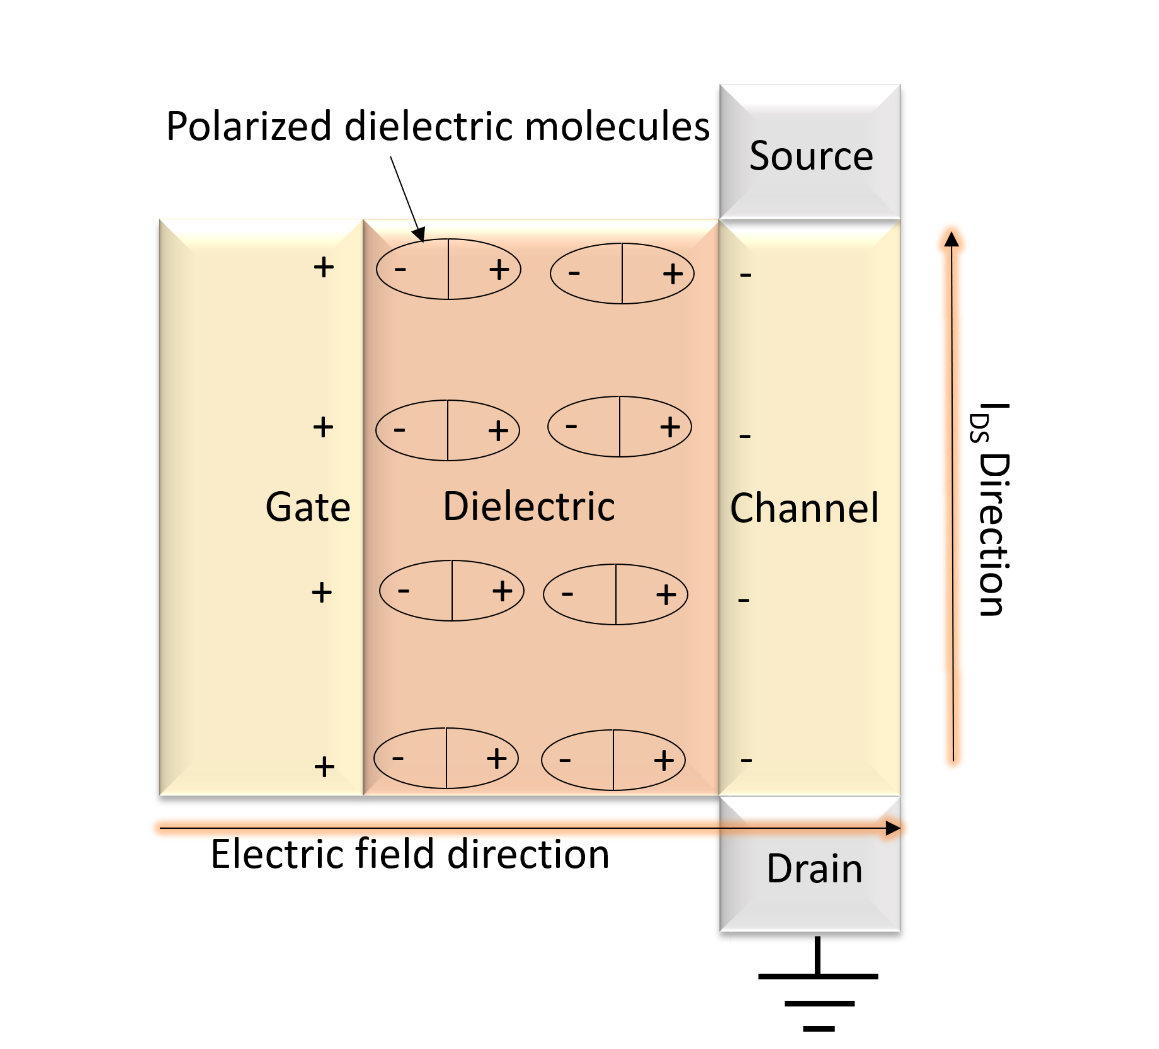
\includegraphics[width=0.7\textwidth]{figures/fig15.png}
\caption[Example of caption.]{A positive voltage applied to the gate of the transistor at the left side and dielectric molecules polarized in a way that capacitor like plates created in both interfaces. negative charge carriers accumulation in interface at right side make a channel which leads the current from drain to source.\label{fig15}}
\end{figure}


The combination of a large gate capacitance per unit area due to the CSPE and a high field-effect mobility of the semiconductor allows EGFETs to generate drain currents (ID) ranging from hundreds of µA to mA at low operating voltages (≤ 1.5 V)~\cite{ref80}.

Inkjet-printed EGFETs typically operate at frequencies ranging from several tens of Hz up to kHz ~\cite{ref77},~\cite{ref78}.



\section{Exploration of Logic Designs}
Since EGFET technology is relatively new, there is limited prior research on its circuit and logic-level implementations. Existing work mainly focuses on constructing digital components like NAND, NOR, or XOR logic gates, along with inverter.
Inverters represent the fundamental building blocks of digital electronics. Here in the table \ref{tab4} different works based on low voltage inverter circuit has been compared.
This review provides an
overview of inverter operation and considers all aspects of such circuits including organic/inorganic inverters, architectures and threshold voltage in recent years.

table 
\begin{table}[h]
\centering
\caption{circuit operation using different inverter. The DTBDT-C6 stands for utilizing a blend of 2,7-dihexyl-dithieno[2,3-d:2′,3′-d′]benzo[1,2-b:4,5-b′]dithiophene and polystyrene. The nameTIPS-pentacene is the abbreviation of 6,13-Bis (triisopropylsilylethynyl)pentacene. ThediF-TES-ADT is made of 2,8-difluoro-5,11-bis(triethylsilylethynyl)anthradith-iophene  (diF-TES-ADT)  and  polystyrene  (PS),  which  is  known  as  a  high-performance  p-type  channel  material  patternable  with  inkjet  printing. The TU-3 blended ink consisting of a 4,8-bis[5-(3-cyanophenyl)thiophene-2-yl]benzo[1,2-c:4,5-c’]bis[1,2,5]thiadiazole     derivative     (TU-3)     and  poly(α-methylstyrene)  (PαMS). (SWCNT) indium oxide/single-walled carbon nanotube. The SWCNT is semi-conducting single-walled carbon nanotubes  }
\begin{tabular}{|c|c|c|c|c|c|c|c|c|}
\hline
Channel&type&$V_{th} [V]$&W[ \mu m]/L[ \mu m]&Supply voltage&gain&ref&year\\
\hline
DTBDT-C6&Organic&-0.2&780/8&0.5&10&\cite{ref29}&2017\\
\hline
TIPS-pentacene&Organic&−1.2&247/47&-40&7.8&\cite{ref30}&2011\\ 
\hline
DTBDT-C6&Organic&0.35&1070/9&-5&100&\cite{ref31}&2016\\
\hline
diF-TES-ADT&Organic p-type&0.6&100/50&10&14&\cite{ref32}&2017\\
\hline
TU-3&Organic n-type&2.7&600/50&10&14&\cite{ref32}&2017\\
\hline
DPPDTT&Organic n-type&-9&50/150&40&8&\cite{ref33}&2022\\
\hline
$In_2O_3$&Inorganic&0.2&60/150&1&3.5&\cite{ref34}&2020\\
\hline
PEDOT:PSS&Organic&0.1&150/80&4.83&13.93& ~\cite{ref35}&2021\\
\hline


SWCNT&Inorganic&0.5&-&0-1&$10$ at $V_{DD}$$=0.7$& ~\cite{ref38}&2022\\
\hline
TIPS-Pentacene&Organic&-&-&0.99&6.7& ~\cite{ref37}&2019\\
\hline



\end{tabular}
\label{tab4}
\end{table}


